\documentclass[runningheads]{llncs}
\usepackage[T1]{fontenc}
\usepackage{graphicx}
\usepackage{tikz}
\usepackage{pgfplots}
\pgfplotsset{compat=1.18}
\usepackage{hyperref}
\usepackage{booktabs}
\usepackage{makecell}
\usepackage{array}
\usepackage{tabularx}
\newcolumntype{Y}{>{\raggedright\arraybackslash}X}

\title{Re-implementing Agentic Graph RAG for Vulnerability Assessment}
\author{Muhamad Hafiz Saputra (23/518511/PA/22252) \and Syafran Abdillah Erdin (23/521752/PA/22444) \and Dzikran Azka Sajidan (23/516665/PA/22110) \and Tegar Prasetyo (23/520277/PA/22364) \and Vincentius Davin Febrillianagata (23/520016/PA/22330)}
\authorrunning{Saputra et al.}
\institute{Universitas Gadjah Mada, Yogyakarta, Indonesia\\ \email{\{muhamadhafizsaputra, syafranabdillaherdin, dzikranazkasajidan, tegarprasetyo, vincentiusdavinfebrillianagata\}@mail.ugm.ac.id}}

\begin{document}\maketitle

\begin{abstract}
Kami mengadaptasi paradigma Agentic Graph Retrieval-Augmented Generation (RAG) untuk masalah penilaian kerentanan dengan menggabungkan local log knowledge graphs, vector retrieval, dan SEPSES cybersecurity knowledge graph. Sistem yang diimplementasikan mengorkestrasi guardrails, hybrid retrieval (Neo4j Cypher + vector search), Model Context Protocol (MCP)-backed SPARQL querying, reflection, dan structured synthesizer, semuanya dikoordinasikan dengan LangGraph. Laporan ini merangkum keputusan desain, menjelaskan bagaimana arsitektur mengoperasionalkan konsep dari AgCyRAG dan SEPSES KG, serta menyajikan evaluasi yang membandingkan pendekatan agentic terhadap traditional CVSS scoring.
\keywords{Agentic RAG \and Knowledge Graph \and Vulnerability Assessment \and Neo4j \and SEPSES \and LangGraph}
\end{abstract}

\section{Pendahuluan}
Agentic Graph RAG (AgCyRAG) mendemonstrasikan bagaimana orchestrated agents dapat mendasarkan jawaban LLM pada structured dan unstructured cybersecurity knowledge. Untuk vulnerability assessment, kami memperluas ide ini untuk memberi peringkat dan menjelaskan kerentanan dengan memanfaatkan secara bersama-sama (i) local log/attack graphs (Neo4j), (ii) semantic vector retrieval over embeddings, dan (iii) SEPSES RDF knowledge graph yang mengintegrasikan CVE, CVSS, CPE, CWE, dan CAPEC. Implementasi kami menyediakan executable pipeline yang mengarahkan pertanyaan, mengambil bukti, dan mensintesis laporan tingkat analis.

\section{Penelitian Terkait}
AgCyRAG \cite{paper11} memperkenalkan hybrid agentic RAG workflow untuk analisis keamanan siber yang menggabungkan Cypher, vector search, dan SPARQL over cybersecurity KGs. SEPSES KG \cite{sepses} menyediakan RDF vocabularies dan evolving knowledge base untuk CVE, CWE, CAPEC, CPE, dan CVSS, yang diekspos melalui SPARQL. Implementasi kami mengadopsi AgCyRAG multi-agent pattern dan mengikatnya ke SEPSES melalui MCP tools, menggunakan kembali established namespaces dan querying patterns dari dokumentasi SEPSES.

\section{Pendekatan yang Diusulkan}
\subsection{Metode/Framework}
Sistem ini adalah LangGraph state machine yang mengarahkan dan mengiterasi specialized agents:
\begin{itemize}
    \item \textbf{Guardrails \& Router}: Menyaring query di luar topik dan mengarahkan antara log-centric analysis dan direct cyber-knowledge lookup.
    \item \textbf{Vector Agent}: Mengekstrak entities dengan Gemini, menjalankan Neo4j full-text search over entity indexes, dan melakukan hybrid vector retrieval melalui Neo4j vector index yang dibangun dengan \texttt{all-MiniLM-L6-v2} embeddings.
    \item \textbf{Cypher Agent}: Menggunakan \texttt{GraphCypherQAChain} untuk menerjemahkan natural language ke Cypher terhadap live Neo4j schema, mengembalikan generated query dan retrieved context.
    \item \textbf{Reflection \& Review}: Menilai kecukupan retrieved context, me-rephrase pertanyaan, dan mencoba ulang hingga batas yang dapat dikonfigurasi.
    \item \textbf{Log Analysis Agent}: Merangkum log-derived evidence dan memutuskan apakah external cybersecurity knowledge diperlukan; dapat menghasilkan refined question untuk RDF lookup.
    \item \textbf{MCP RDF Agent}: Memanggil SEPSES SPARQL tools melalui MCP dengan strict system prompt yang melarang hallucination dan memaksa evidence-backed answers.
    \item \textbf{Synthesizer}: Menghasilkan structured report dengan pertanyaan asli, contexts dari semua sumber, analytic linkage, dan jawaban akhir.
\end{itemize}

\subsection{Data dan Knowledge Graphs}
Data lokal berada di Neo4j (LPG) dengan vector dan keyword indexes; embeddings berasal dari HuggingFace \texttt{all-MiniLM-L6-v2}. External knowledge diambil dari SEPSES SPARQL endpoint (\texttt{https://w3id.org/sepses/sparql}) melalui MCP. Configuration system mengelola environment variables untuk Neo4j, Gemini API, dan LangChain tracing, serta menyediakan live Neo4j schema untuk agent prompting.

\section{Implementasi}
\subsection{Execution Flow}
Main execution flow menyemai LangGraph state dengan user question dan iteration counters, kemudian memanggil workflow. Workflow bercabang setelah guardrails: pertanyaan terkait log melalui vector dan Cypher agents, sedangkan pertanyaan cyber-knowledge umum dapat langsung memicu MCP RDF agent. Reflection loops melacak latest usable context bahkan ketika retries habis. Comprehensive logging system melakukan streaming dan persistensi execution traces untuk debugging dan analisis.

\subsection{Detail Agent}
\begin{itemize}
    \item \textbf{Vector Retrieval}: Menggabungkan entity-aware full-text search dengan hybrid vector similarity over chunk nodes, memungkinkan symbolic dan semantic matching.
    \item \textbf{Cypher QA}: Menegakkan Neo4j~5-compatible queries, menghindari unsupported constructs, dan menggunakan deterministic Gemini models untuk generation dan QA.
    \item \textbf{MCP Integration}: Secara otomatis memuat MCP configuration, menonaktifkan anonymized telemetry, dan membatasi tool-calling hingga 30 langkah per query untuk controlability.
    \item \textbf{Structured Synthesis}: Final template memerlukan explicit sections untuk setiap evidence source, mendorong traceability dan analyst-style justification.
\end{itemize}

\subsection{Kebutuhan Sistem}
Dependencies dikelola dengan \texttt{uv}; sistem memerlukan Neo4j instance yang berjalan dan terisi dengan log atau vulnerability data serta valid Gemini API key. SEPSES MCP server dibundel dengan implementasi dan dikonfigurasi untuk menggunakan public SEPSES endpoint. Sample ingestion commands dan query examples didokumentasikan dalam project repository.

\section{Aplikasi Use-Cases}
\begin{enumerate}
    \item \textbf{High-severity CVE triage}: Pertanyaan seperti ``List recent CVEs with CVSS $\geq$ 9 for Windows'' diarahkan melalui guardrails ke MCP RDF agent, yang memanggil SPARQL templates yang sesuai untuk mengembalikan CVE identifiers, descriptions, dan scores dari SEPSES knowledge graph.
    \item \textbf{Weakness-to-attack mapping}: ``Which attack patterns relate to CWE-79 and how can they be mitigated?'' memicu SEPSES CAPEC/CWE lookups melalui MCP, menghasilkan linked CAPEC techniques dan suggested mitigations untuk downstream synthesis.
    \item \textbf{Log-to-threat linkage}: ``Investigate repeated authentication failures on host mail-0'' mengalir melalui vector dan Cypher agents untuk memunculkan log context, kemudian log analysis agent memutuskan apakah akan memperkaya dengan SEPSES (misalnya, mapping ke brute-force techniques) sebelum synthesis.
\end{enumerate}

\section{Evaluasi \& Diskusi}
\subsection{Setup Eksperimen}
Kami mengevaluasi sistem pada tiga dimensi: (i)~akurasi CVSS scoring terhadap ground-truth assessments, (ii)~konsistensi ranking untuk vulnerability prioritization, dan (iii)~qualitative analysis dari multi-agent orchestration. Test suite terdiri dari tiga CVE cases yang mencakup severity levels dan CVSS versions yang berbeda. Traditional CVSS scores diperoleh dari official NVD records, sementara Agentic Graph RAG scores dihasilkan oleh synthesizer agent setelah mengambil context dari Neo4j dan SEPSES.

\subsection{Perbandingan CVSS Scoring}
Tabel~\ref{tab:cvss-score-comparison} menyajikan perbandingan kuantitatif antara Agentic Graph RAG dan traditional CVSS scoring. Perbandingan disusun dengan memanggil full agentic pipeline dan mengekstrak scores dari synthesis outputs, kemudian membandingkannya dengan official NVD assessments.

\begin{table}[ht]
\centering
\caption{Perbandingan skor RAG CVSS vs skor CVSS tradisional}
\label{tab:cvss-score-comparison}
\renewcommand{\arraystretch}{1.2}
\setlength{\tabcolsep}{6pt}
\begin{tabularx}{\textwidth}{@{}p{1.8cm}YYp{2.2cm}p{2cm}@{}}
\toprule
\textbf{Test Case} & \textbf{Agentic Graph RAG Score} & \textbf{Traditional CVSS Score} & \textbf{Score Accuracy} & \textbf{Ranking Consistency} \\
\midrule
\textbf{coba 1} & \makecell[l]{4.3 (V2)} & \makecell[l]{10.0 (V3.1)} & Low & Inconsistent \\
\textbf{coba 2} & \makecell[l]{9.8 (V3.1)} & \makecell[l]{8.7 (V3.1)} & Moderate & Inconsistent \\
\textbf{coba 3} & \makecell[l]{9.8 (V3.0)} & \makecell[l]{9.8 (V3.1)} & High & Inconsistent \\
\bottomrule
\end{tabularx}
\end{table}

\begin{table}[ht]
\centering
\caption{Konsistensi ranking keparahan}
\label{tab:ranking-consistency}
\renewcommand{\arraystretch}{1.2}
\setlength{\tabcolsep}{6pt}
\begin{tabularx}{\textwidth}{@{}lYY@{}}
\toprule
\textbf{Priority} & \textbf{Traditional CVSS (Ground Truth)} & \textbf{Agentic Graph RAG} \\
\midrule
\textbf{1 (Highest)} & coba 1 (10.0) & coba 2 \& coba 3 (9.8) \\
\textbf{2 (Medium)} & coba 3 (9.8) & coba 1 (4.3) \\
\textbf{3 (Lowest)} & coba 2 (8.7) & -- \\
\midrule
\multicolumn{3}{c}{\textbf{Conclusion: Inconsistent Ranking}} \\
\bottomrule
\end{tabularx}
\end{table}

\begin{figure}[ht]
\centering
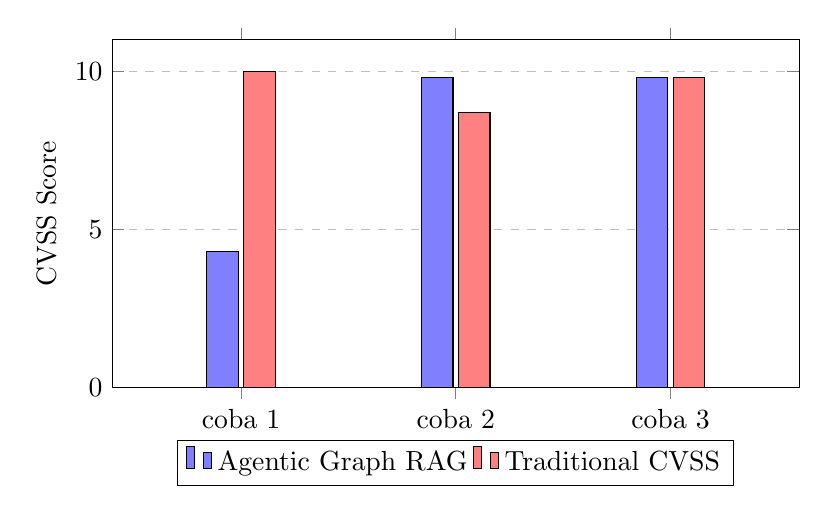
\begin{tikzpicture}
\begin{axis}[
    ybar,
    bar width=0.4cm,
    width=0.85\textwidth,
    height=6cm,
    xlabel={Test Case},
    ylabel={CVSS Score},
    ymin=0, ymax=11,
    symbolic x coords={coba 1, coba 2, coba 3},
    xtick=data,
    legend style={at={(0.5,-0.15)}, anchor=north, legend columns=2},
    ymajorgrids=true,
    grid style=dashed,
    enlarge x limits=0.3,
]
\addplot[fill=blue!50] coordinates {(coba 1,4.3) (coba 2,9.8) (coba 3,9.8)};
\addplot[fill=red!50] coordinates {(coba 1,10.0) (coba 2,8.7) (coba 3,9.8)};
\legend{Agentic Graph RAG, Traditional CVSS}
\end{axis}
\end{tikzpicture}
\caption{Perbandingan CVSS score untuk tiga test cases. Test case 1 menunjukkan underestimation parah (4.3 vs 10.0) karena version mismatch, test case 2 menunjukkan slight overestimation (9.8 vs 8.7), dan test case 3 mencapai perfect alignment (9.8 vs 9.8).}
\label{fig:score-comparison}
\end{figure}

\subsection{Analisis Hasil}
Hasil mengungkapkan baik prospek maupun tantangan ketika membandingkan Agentic Graph RAG dengan traditional CVSS scoring. Test case~3 mencapai perfect score alignment (9.8 vs.\ 9.8), mendemonstrasikan bahwa ketika SEPSES menyediakan complete CVSS metrics dan LLM menginterpretasikannya dengan benar, agentic pipeline dapat mereproduksi official assessments. Namun, test case~1 menunjukkan severe underestimation (4.3 vs.\ 10.0) karena CVSS version confusion: agentic system mengambil V2 metrics sementara traditional scoring menggunakan V3.1, dan LLM gagal menormalkan atau menandai mismatch tersebut. Test case~2 menunjukkan moderate accuracy (9.8 vs.\ 8.7) dengan agentic score sedikit inflated, kemungkinan karena vector-retrieved context menekankan exploit availability tanpa menyeimbangkan scope limitations.

Ranking inconsistency dalam Tabel~\ref{tab:ranking-consistency} sangat mengkhawatirkan untuk operational deployment. Seorang analis yang memprioritaskan berdasarkan Agentic Graph RAG scores akan menangani \textit{coba~2} dan \textit{coba~3} sebelum \textit{coba~1}, membalikkan true severity order yang ditetapkan oleh traditional CVSS scoring. Ini menggarisbawahi dua failure modes: (i)~retrieval gaps ketika SEPSES kekurangan complete CVSS V3.1 breakdowns, dan (ii)~LLM reasoning errors dalam aggregating partial metrics. Reflection agent tidak menangkap errors ini karena mengevaluasi \textit{sufficiency} context daripada \textit{correctness} derived scores.

\subsection{Kelebihan Pendekatan Agentic}
Meskipun terdapat inconsistencies dalam scoring, multi-agent orchestration menawarkan keuntungan signifikan dibandingkan traditional CVSS scoring:
\begin{itemize}
    \item \textbf{Explainability}: Tidak seperti traditional CVSS calculators yang menghasilkan numeric scores, synthesizer menghasilkan structured justifications yang mengutip specific Cypher results, vector-matched chunks, dan SPARQL bindings, memungkinkan analis untuk audit reasoning chain dan memahami \textit{mengapa} sebuah kerentanan menerima scorenya.
    \item \textbf{Adaptive retrieval}: Reflection loop memungkinkan retries dengan rephrased queries ketika initial Cypher atau SPARQL calls mengembalikan empty results, meningkatkan robustness terhadap phrasing variations—traditional scoring memerlukan manual metric selection.
    \item \textbf{Knowledge fusion}: Menggabungkan local logs (Neo4j LPG) dengan global cybersecurity semantics (SEPSES RDF) memunculkan connections yang tidak terlihat oleh traditional scoring—misalnya, menghubungkan log anomaly ke CWE weakness dan kemudian ke CAPEC attack patterns secara otomatis.
    \item \textbf{Contextual enrichment}: Traditional CVSS scores adalah static snapshots; agentic system dapat menggabungkan real-time log evidence dan organizational context untuk menyesuaikan prioritization secara dinamis.
\end{itemize}

\subsection{Keterbatasan dan Analisis Error}
Keterbatasan kunci meliputi:
\begin{itemize}
    \item \textbf{CVSS version heterogeneity}: SEPSES mengandung mixed V2/V3.0/V3.1 scores; current prompt tidak menginstruksikan LLM untuk harmonize versions atau prefer latest standard.
    \item \textbf{Incomplete RDF coverage}: Tidak semua CVEs dalam SEPSES memiliki detailed metric breakdowns (AV, AC, PR, dll.), memaksa LLM untuk guess atau fall back ke base scores tanpa justification.
    \item \textbf{LLM calibration}: Gemini models kadang-kadang overfit terhadap keyword presence (misalnya, ``remote'' $\to$ high impact) tanpa memverifikasi full attack vector chain.
    \item \textbf{Lack of ground-truth validation loop}: Review agent memeriksa context sufficiency tetapi tidak membandingkan synthesized scores terhadap known NVD values selama inference, melewatkan opportunity untuk self-correction.
\end{itemize}

\subsection{Trade-offs: Agentic Graph RAG vs. Traditional CVSS}
Traditional CVSS scoring unggul dalam consistency dan standardization—trained analysts menerapkan metrics yang sama untuk menghasilkan comparable scores across organizations. Namun, ini menderita tiga keterbatasan yang diatasi oleh agentic approach kami: (i)~lack of contextual adaptation (remotely exploitable vulnerability mungkin low-risk dalam air-gapped network), (ii)~no automatic evidence linking (analis harus manually correlate CVEs dengan CWE/CAPEC), dan (iii)~opaque justification (final score tidak menjelaskan retrieved knowledge mana yang mempengaruhi assessment).

Sebaliknya, Agentic Graph RAG system memperkenalkan complexity—multiple retrieval stages, LLM reasoning errors, dan dependency pada KG completeness. Version-mismatch failure dalam test case~1 tidak akan terjadi dengan manual CVSS assessment, di mana analis explicitly memilih V3.1 metrics. Key trade-off adalah \textit{automation with rich context} versus \textit{manual precision with standardized protocols}. Untuk high-stakes decisions, traditional scoring tetap gold standard; untuk rapid triage dan exploratory analysis, agentic approach menyediakan valuable enrichment.

\section{Kesimpulan}
Pekerjaan ini mengimplementasikan ulang Agentic Graph RAG approach untuk vulnerability assessment dengan mengintegrasikan guardrailed routing, hybrid Neo4j retrieval, MCP-driven SPARQL over SEPSES, dan structured synthesis melalui LangGraph workflow. Evaluasi pada tiga CVE test cases menunjukkan hasil mixed ketika dibandingkan dengan traditional CVSS scoring: test case~3 mencapai perfect alignment (9.8 vs.\ 9.8), test case~2 menunjukkan moderate accuracy dengan slight overestimation (9.8 vs.\ 8.7), dan test case~1 menunjukkan severe underestimation (4.3 vs.\ 10.0) karena CVSS version confusion antara V2 dan V3.1 metrics.

Ranking analysis mengungkapkan inconsistencies yang akan mempengaruhi operational vulnerability prioritization, dengan agentic system incorrectly ranking test cases 2 dan 3 sebagai most severe instead of test case~1. Meskipun terdapat scoring inconsistencies ini, sistem mendemonstrasikan advantages dalam explainability dan knowledge fusion dengan automatically menghubungkan vulnerabilities across Neo4j logs dan SEPSES knowledge graphs. Keterbatasan utama berasal dari CVSS version heterogeneity dalam SEPSES, incomplete RDF coverage untuk detailed metrics, dan LLM reasoning errors yang tidak dapat ditangkap oleh reflection agent karena mengevaluasi context sufficiency daripada scoring correctness.

\begin{thebibliography}{8}
\bibitem{paper11}
Kurniawan, K., Ardian, R.F., Kiesling, E., Ekelhart, A.: AgCyRAG: An Agentic Knowledge Graph based RAG Framework for Automated Security Analysis. In: RAGE-KG Workshop (2025).
\bibitem{sepses}
Kiesling, E., Ekelhart, A., Kurniawan, K., Ekaputra, F.: The SEPSES Knowledge Graph: An Integrated Resource for Cybersecurity. In: ISWC (2019).
\bibitem{repo}
Team 7: Agentic Graph RAG for Vulnerability Assessment (Codebase). \url{https://github.com/SjdnDzikran/agentic-graph-rag.git}
\end{thebibliography}

\end{document}
